Let us suppose the finite states $s1,s2,s3,s4$. In zero-sum games $U(s,1)=-U(s,2)$ or $\sum_{k}^{N}U(s,k)=0$ sum of the utilities of all the players is zero for all states. For simplicity, let $U(s)=[U(s,1),U(s,2)]$.


\subsubsection{}
For the sake of the reasoning, we will assume that player 2 is optimal and that the following values represent the final utilities of the four states for each player:
\begin{align*}
    U(s1)&=[1,1] \\
    U(s2)&=[5,-3] \\
    U(s3)&=[0,0] \\
    U(s4)&=[1,-1]
\end{align*}

The diagram in Fig. \ref{fig:5_a} shows the corresponding non-zero sum game.
\begin{figure}[h]
    \centering
    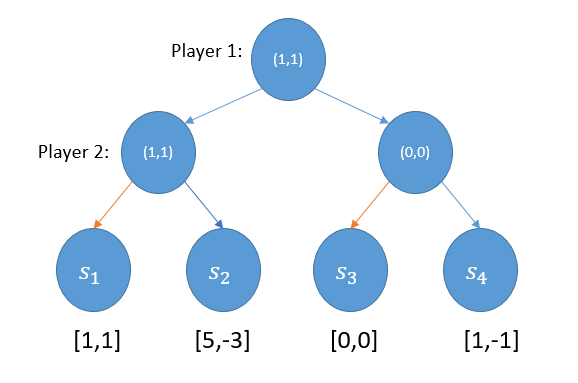
\includegraphics[width=0.6\linewidth]{5_a}
    \caption{Example of a non-zero sum game where the optimality of minimax holds.}
    \label{fig:5_a}
\end{figure}

In the example of Fig. \ref{fig:5_a}, minimax still returns the optimal value and the optimal move. Minimax is optimal because there is a negative correlation between the two players i.e. what is good for player 1 is bad for player 2. Player 1 can see that, for the opponent's optimal moves, the game can terminate either in state $[1,1]$ or in state $[0,0]$: indeed, player's 2 best moves are represented by the edges leaning to left in both cases (orange arrows). So minimizing player's 1 utility in the opponent move nodes was the same as maximize opponent utility. Hence, minimax is optimal in such an example.

\subsubsection{}
We now assume that the following values represent the final utilities of the four states for each player:
\begin{align*}
    U(s1)&=[1,1] \\
    U(s2)&=[-1,-1] \\
    U(s3)&=[2,0.5] \\
    U(s4)&=[-1.5,0]
\end{align*}

The diagram in Fig. \ref{fig:7_c_first} shows the corresponding non-zero sum game.
\begin{figure}[h]
    \centering
    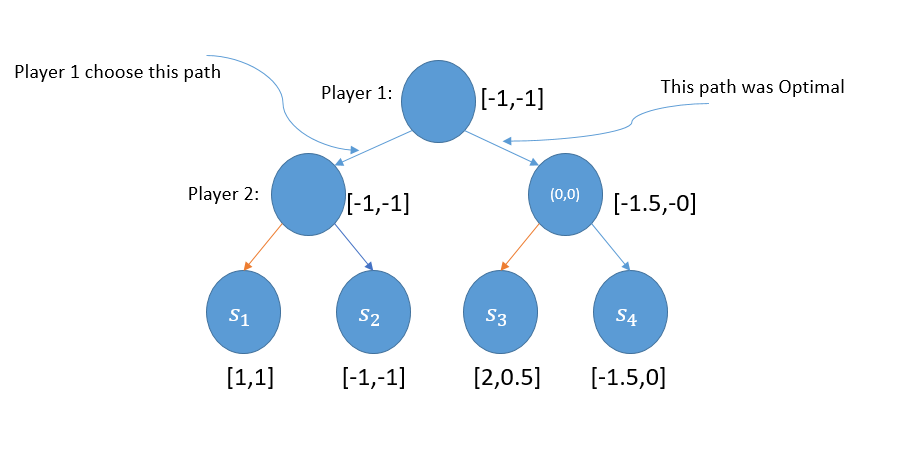
\includegraphics[width=0.8\linewidth]{7_c}
    \caption{Example of a non-zero sum game where the optimality of minimax does no hold.}
    \label{fig:7_c_first}
\end{figure}

The example in Fig. \ref{fig:7_c_first} shows a case where minimax is not optimal, i.e. does not perform the best moves. Minimax minimizes the utility of player 1 at the opponent nodes, but the optimal path instead would be given if it tried to maximize the opponents utility at the opponent's nodes.

Considering the specific example under the scope, the minimax algorithm would compute $[-1,-1]$ and $[-1.5,0]$ and would therefore chose to go left and get minimax value of $-1$, instead of $-1.5$. However, the opponent goes left in his nodes (orange arrows) during its turn, because that is how it can maximizes its terminal utility. Thus, considering this game-play, player 1 will get the terminal utility of 1. After a deeper analysis, the best move for player 1 was to go right, because then the opponent will take the lest node $[2,0.5]$ and player 1 terminal utility could be 2.
